\author{Andriy Zatserklyaniy, zatserkl@fnal.gov}
\documentclass[english]{article}
\usepackage{babel}
\usepackage{amsmath}
\usepackage[T1]{fontenc}
\usepackage[latin9]{inputenc}   % encoding ISO-8859-9
\usepackage{graphicx}
\usepackage{esint}              % integral symbols
\usepackage{parskip}            % for \smallskip, \medskip and \bigskip
\usepackage{cancel}             % to cancel out variables in text
\usepackage[active]{srcltx}     % enables reverse search by Shift-LeftClick in dvi file
\usepackage{listings}		% to include C++ code

%-- function to scale pictures --%
\makeatletter
\def\ScaleIfNeeded{%
\ifdim\Gin@nat@width>\linewidth
\linewidth
\else
\Gin@nat@width
\fi
}

\begin{document}

\title{Proton energy and range}

\maketitle

\section{Proton energy at depth x}

Proton stopping power may be approximate by expression 

\begin{align*}
\frac{dE}{dx} = -247.93 E^{-0.7637} \hspace{0.5cm} \frac{MeV}{g/cm^2}
\end{align*}

Rewrite and solve this differential equation. 

\begin{align*}
\frac{dE(x)}{dx} = s(E) = -aE^{-b}
\end{align*}

In terms of $y(x) = E(x)$

\begin{align*}
\frac{dy(x)}{dx} = f(y)
\end{align*}

where $y(x) = E(x)$ and $f(y) = s(E)$

Separate the variables

\begin{align*}
\frac{dy}{f(y)} = dx
\end{align*}

Integrate the equation

\begin{align*}
x = -\int \frac{dy}{ay^{-b}} + C
\end{align*}

\begin{align*}
x = - \frac{y^{b+1}}{a(b+1)} + C
\end{align*}

Initial condition is that proton has energy $E$ at depth $x$:

\begin{align*}
& 0 = - \frac{E_0^{b+1}}{a(b+1)} + C \\
& C = \frac{E_0^{b+1}}{a(b+1)}
\end{align*}

and

\begin{align*}
& x = \frac{E_0^{b+1}}{a(b+1)} - \frac{y^{b+1}}{a(b+1)} \\
& y = \Bigl( E_0^{b+1} - a(b+1)x \Bigr)^\frac{1}{b+1}
\end{align*}

Finally,

\begin{align}
E = \Bigl( E_0^{b+1} - a(b+1)x \Bigr)^\frac{1}{b+1} \label{eq:E_vs_x}
\end{align}

or

\begin{align*}
E(x) = \Bigl( E_0^{1.7637} - 247.93 \cdot 1.7637 \cdot x \Bigr)^{\dfrac{1}{1.7637}}
\end{align*}

See plot on the Fig.\ref{fig:T_vs_x}.

Example: If we installed polystyrene degrader $(\rho = 1.05~g/cm^3)$ with thickness of 200~$mm$ in front of the scintillator block, the proton will exit it with kinetic energy of about 80~$MeV$. This energy will be deposited in the scintillator block.  

% The ROOT command line is
% 
% TF1* fEx = new TF1("fEx", "pow(pow([0],1+[2])-[1]*(1+[2])*(0.1*x), 1./(1+[2]));proton path, mm;T\_{proton}, MeV", 0,262);
% 
% fEx->SetParameters(200,247.93,0.7637)

\begin{figure}[h]
\centering
% \begin{minipage}[t]{0.75 \linewidth}
\begin{minipage}[t]{1.0 \linewidth}
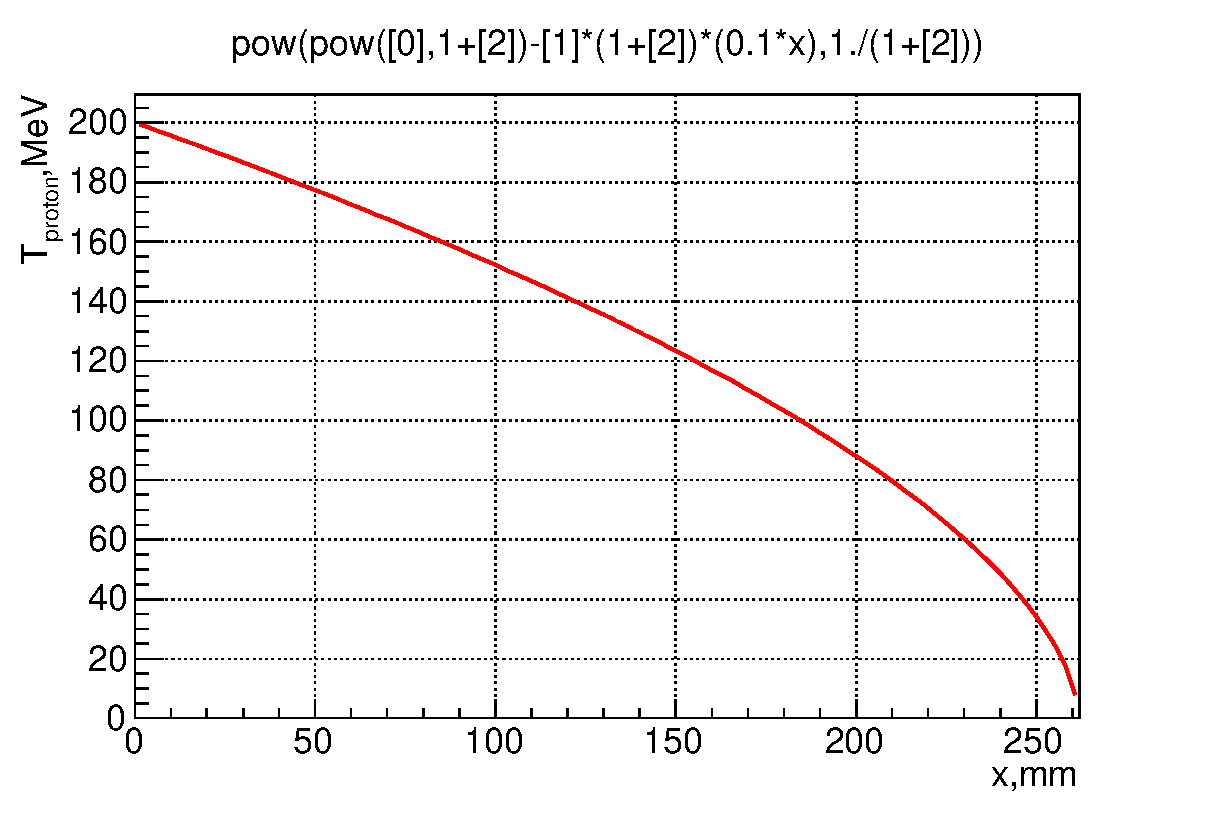
\includegraphics[width=\ScaleIfNeeded]{Proton_energy_vs_path_length}
\caption{Kinetic energy of proton with initial energy 200 MeV vs depth}
\label{fig:T_vs_x}
\end{minipage}
\end{figure}

\section{Proton Range}

\begin{align*}
R(E) &= \int_0^E \frac{dE}{dE/dx} \\
&= \int_0^E\frac{dE}{aE^{-b}} \\
&= \frac{1}{a} \int_0^E E^b dE \\
&= \frac{E^{b+1}}{a(b+1)} \\
&= \frac{E^{1.7637}}{247.93 \cdot 1.7637}
\end{align*}

See result in the Fig.\ref{fig:Proton_Range}.

% Correspondent ROOT expression is 
% 
% F1* fR = new TF1("fR", "10.*pow(x,1+[1])/([0]*(1+[1]));T\_{proton}, MeV;R, mm", 0,200);
% 
% fR->SetParameters(247.93,0.7637)

\begin{figure}[h]
\centering
% \begin{minipage}[t]{0.75 \linewidth}
\begin{minipage}[t]{1.0 \linewidth}
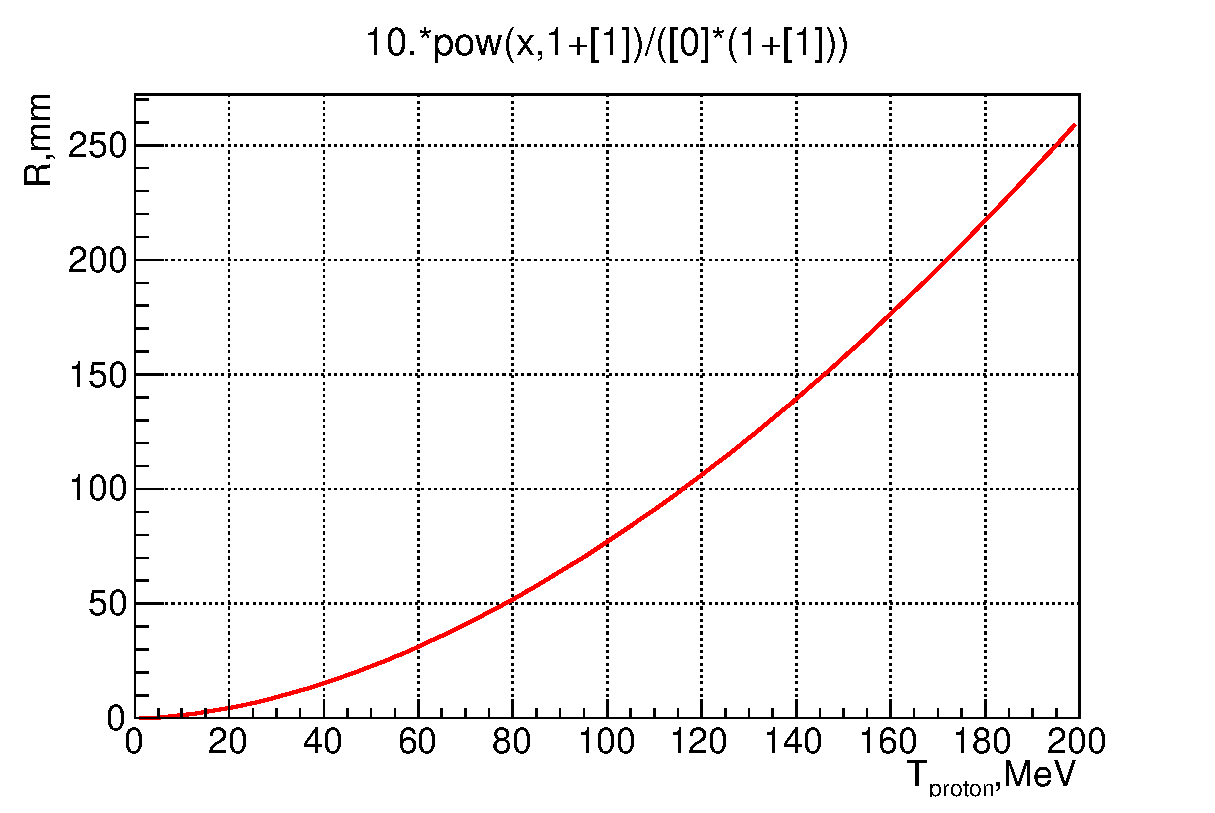
\includegraphics[width=\ScaleIfNeeded]{Proton_Range_vs_T}
\caption{Proton range vs initial energy}
\label{fig:Proton_Range}
\end{minipage}
\end{figure}

Fig.\ref{fig:dEdx_vs_E} shows standard dependence of the $dE/dx$ vs $E$, while the Fig.\ref{fig:dEdx_vs_E} plots dependence of the $dE/dx$ on $x$, derivative of the expression \ref{eq:E_vs_x}.

% TF1* fdEdx = new TF1("fdEdx", "[0]*pow(x,-[1]);E, MeV;dE/dx", 1,100); fdEdx->SetParameters(247.93,0.7637)

% TF1* fdEdxx = new TF1("fdEdxx", "[1]*pow(pow([0],1+[2])-[1]*(1+[2])*(0.1*x), -[2]/(1+[2])); x, mm; dE/dx, MeV/cm", 0,262);   fdEdxx->SetParameters(200,247.93,0.7637)

\begin{figure}[h]
\centering
% \begin{minipage}[t]{0.75 \linewidth}
\begin{minipage}[t]{1.0 \linewidth}
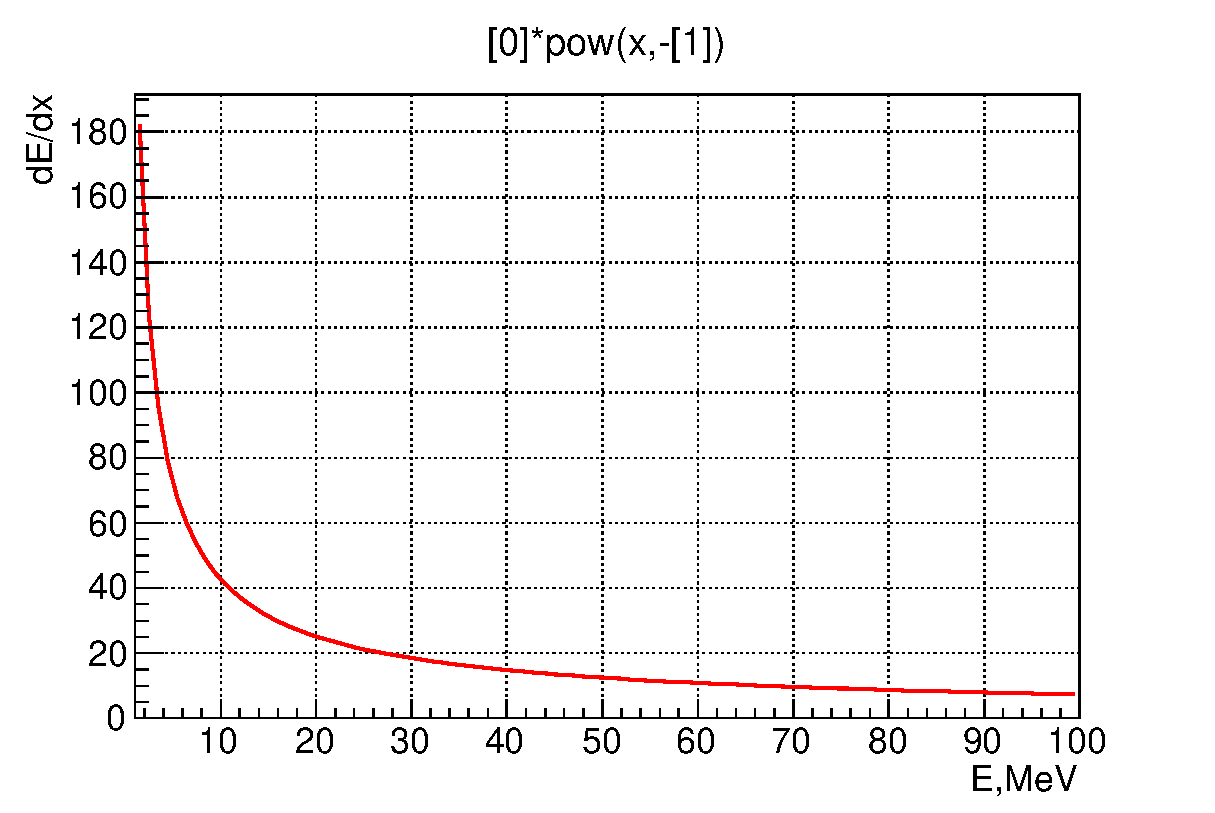
\includegraphics[width=\ScaleIfNeeded]{dEdx_vs_E}
\caption{$dE/dx$ vs $E$}
\label{fig:dEdx_vs_E}
\end{minipage}
\end{figure}

\begin{figure}[h]
\centering
% \begin{minipage}[t]{0.75 \linewidth}
\begin{minipage}[t]{1.0 \linewidth}
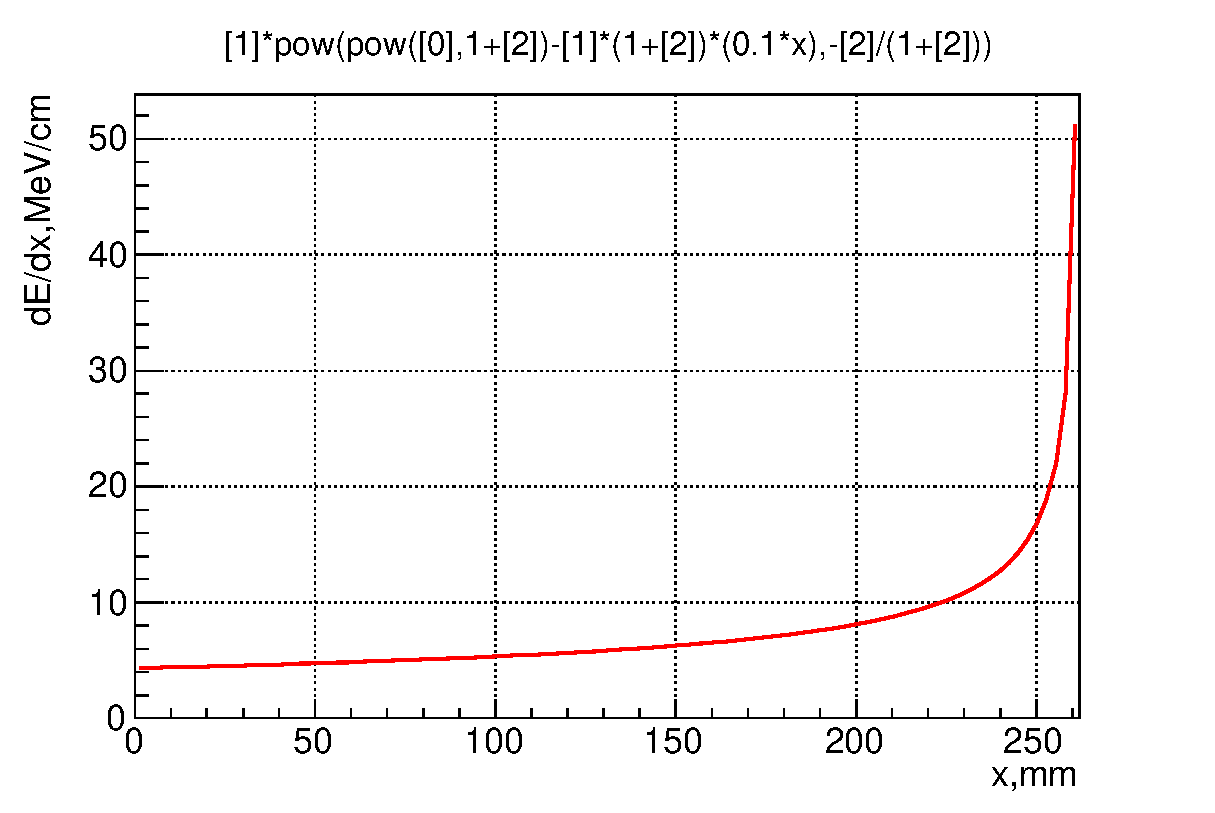
\includegraphics[width=\ScaleIfNeeded]{dEdx_vs_x}
\caption{$dE/dx$ vs $x$}
\label{fig:dEdx_vs_x}
\end{minipage}
\end{figure}

\end{document}
